\vspace{-20pt}

\begin{figure}[h]
    \centering    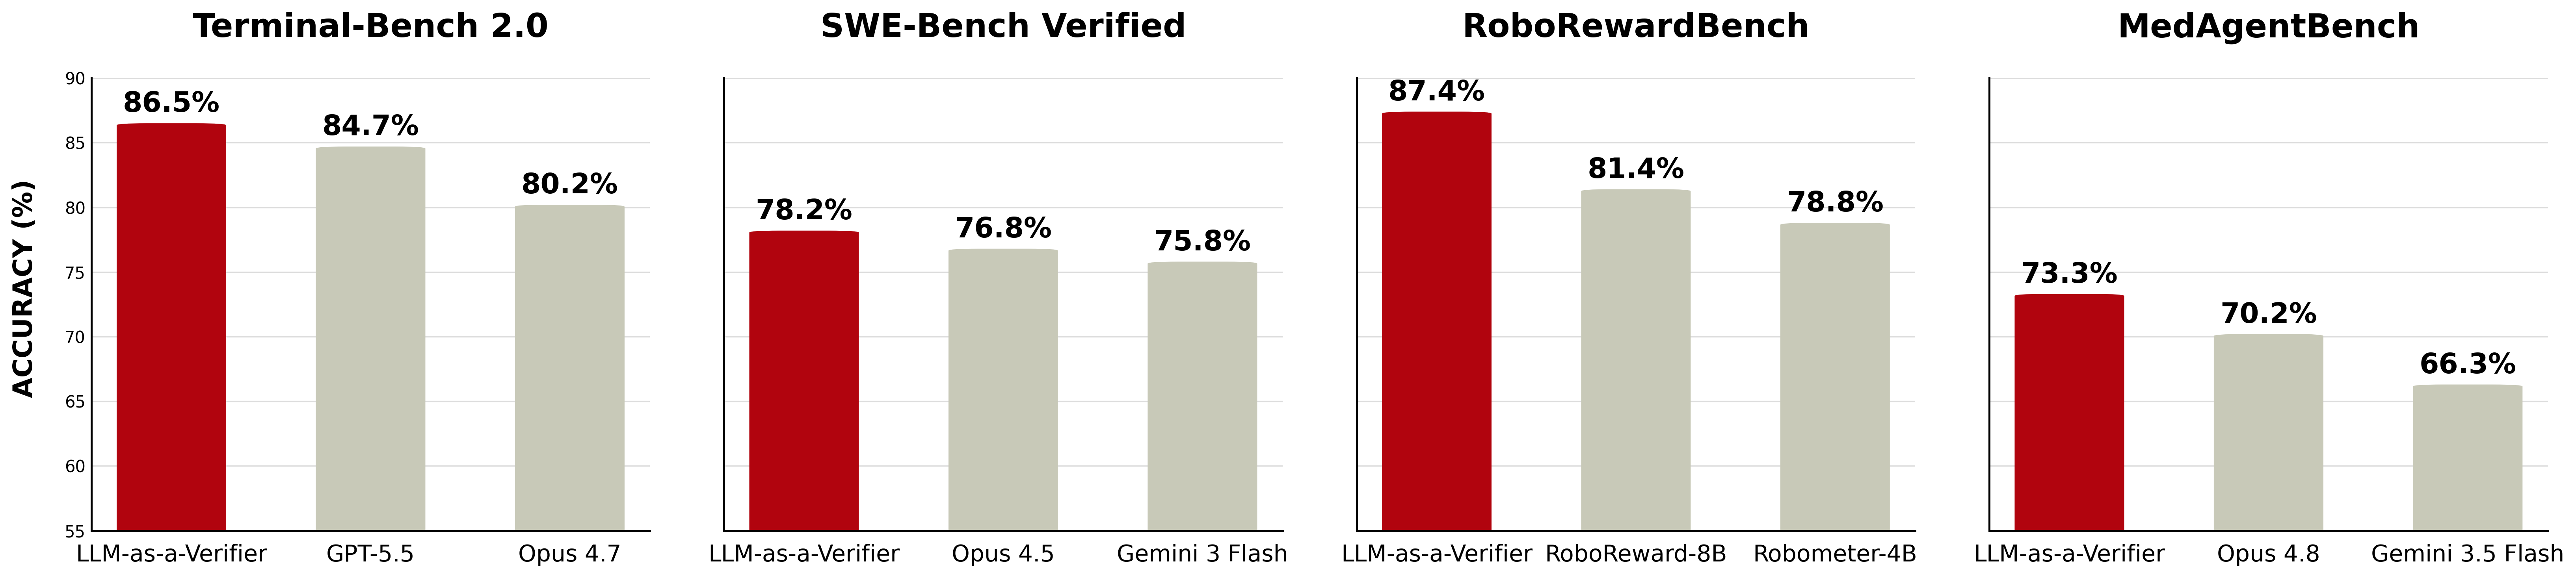
\includegraphics[width=\linewidth]{figures/SOTA.png}
    \caption{\textbf{Overall Performance Results.} Our proposed framework, \textbf{LLM-as-a-Verifier}, achieves state-of-the-art performance across coding, robotics, and medical domains: Terminal-Bench V2 (86.5\%), SWE-Bench Verified (78.2\%), RoboRewardBench (87.4\%), and MedAgentBench (73.3\%).}
    \label{fig:teaser}
\end{figure}

\vspace{4pt}

{\absfont \noindent\textbf{Abstract:} Scaling pre-training, post-training, and test-time compute have become the central paradigms for improving the capabilities of large language models (LLMs). In this work, we identify verification—the ability to determine the correctness of a solution—as a new scaling axis. To unlock this and demonstrate its effectiveness, we introduce LLM-as-a-Verifier, a general-purpose verification framework that provides fine-grained feedback for agentic tasks without requiring additional training. Unlike standard LM judges that prompt LLMs to produce discrete scores for candidate solutions, LLM-as-a-Verifier computes the expectation over the distribution of scoring token logits to generate continuous scores. This probabilistic formulation substantially reduces tie rates when comparing complex solutions and enables verification to scale along multiple dimensions: (1) score granularity, (2) repeated evaluation, and (3) criteria decomposition. In particular, we show that scaling the scoring granularity leads to better separation between positive and negative solutions, resulting in more calibrated comparisons. Moreover, scaling repeated evaluation and criteria decomposition consistently leads to additional gains in verification accuracy through variance and complexity reduction. To make verification scaling practical, we further introduce a cost-efficient ranking algorithm for selecting the best solution among candidates using the preference probabilities derived from the verifier's continuous scores. LLM-as-a-Verifier is effective across coding, robotics, and medical domains. It achieves state-of-the-art performance on Terminal-Bench V2 (86.5\%), SWE-Bench Verified (78.2\%), RoboRewardBench (87.4\%), and MedAgentBench (73.3\%). Beyond verification, the fine-grained signals from LLM-as-a-Verifier can also serve as a proxy for estimating task progress. We build extensions for Claude Code and Codex, enabling developers to monitor and improve their own agentic systems. Finally, we show that LLM-as-a-Verifier can be used as a dense reward signal for RL, improving the sample efficiency of SAC and GRPO on robotics and mathematical reasoning benchmarks. \par} 
\clearpage
